\chapter{Antecedentes y soluciones existentes}
\label{ch:antecedentes}

% Este capítulo cubre el apartado "Antecedentes" de la guía: análisis comparativo
% de soluciones existentes y relación con los objetivos del proyecto.

\section{Situación actual}
\label{sec:situacion_actual}

En la práctica, el problema que aborda Harmony Hub se resuelve hoy de forma fragmentada. Cuando una persona quiere usar la música para concentrarse, bajar el nivel de activación, sentirse acompañada o simplemente atravesar mejor un momento concreto del día, suele recurrir a tres caminos habituales.

El primero consiste en apoyarse en plataformas generalistas de streaming musical, como Spotify, que ofrecen listas personalizadas generadas algorítmicamente a partir del historial de escucha, los temas que se guardan, el momento de uso y los patrones de usuarios con gustos similares \cite{spotify_playlists}. Este enfoque funciona muy bien para descubrimiento y afinidad musical, pero su lógica principal sigue estando ligada a los hábitos de consumo y no a una lectura explícita del estado emocional o de la necesidad puntual del usuario.

El segundo camino se encuentra en aplicaciones de bienestar digital orientadas a foco, relajación o sueño. Herramientas como Endel, Brain.fm o Headspace proponen experiencias sonoras o musicales para ayudar a entrar en ciertos estados de atención, descanso o calma \cite{endel_technology,brainfm_official,headspace_focus}. Aquí el acento ya no está tanto en ``qué música te gusta'', sino en ``qué estado quieres favorecer''. Ese enfoque las aproxima al problema que aborda Harmony Hub.

Sin embargo, la situación actual deja un hueco interesante. Por un lado, las plataformas de streaming tienen un catálogo inmenso y una integración natural con la escucha real del usuario, pero no suelen empezar con un check-in emocional breve ni cerrar el ciclo con una recogida estructurada de feedback sobre la utilidad de la sesión. Por otro, las aplicaciones de bienestar suelen ofrecer audio funcional o contenido guiado, aunque normalmente dentro de ecosistemas cerrados, con menor relación con la biblioteca musical cotidiana del usuario o con sus cuentas de streaming. Esta lectura comparativa es una inferencia a partir de las funcionalidades públicas revisadas en cada solución.

Por tanto, el contexto actual no muestra una ausencia de herramientas, sino más bien una dispersión de enfoques. Existen soluciones potentes para descubrir música, para mejorar el descanso, para facilitar el foco o para construir rutinas de bienestar. Lo que resulta menos frecuente es encontrar una propuesta que una, en una misma experiencia, bienestar cotidiano, contexto inmediato, personalización musical reproducible y aprendizaje progresivo a partir del uso.

\section{Soluciones relacionadas}
\label{sec:soluciones_relacionadas}

Entre las soluciones más relacionadas con Harmony Hub pueden señalarse cuatro referencias especialmente útiles para entender el espacio de diseño del proyecto.

\textbf{Spotify}. Spotify representa el referente más claro en personalización musical a gran escala. Según su propia documentación, sus playlists personalizadas se construyen con algoritmos que consideran qué escucha la persona, cuándo lo escucha, qué canciones guarda y qué patrones presentan usuarios con gustos parecidos \cite{spotify_playlists}. Además, la compañía subraya que su personalización busca ofrecer el contenido adecuado en el momento adecuado, combinando señales algorítmicas y criterio editorial \cite{spotify_responsible_recs}. Su principal fortaleza es, por tanto, la afinidad musical y la capacidad de descubrimiento. No obstante,  su enfoque no se encuentra centrado en un check-in explícito de bienestar o regulación emocional, sino en la evolución del gusto y del comportamiento de escucha. Esta última idea es una inferencia razonable a partir de la forma en que Spotify presenta sus sistemas de personalización.

\textbf{Endel}. Endel se sitúa en un terreno distinto: no trabaja tanto con canciones concretas como con soundscapes adaptativos. Su tecnología declara usar entradas del usuario y del entorno, como la hora del día, el tiempo, el movimiento o determinados sensores, para generar sonido personalizado en tiempo real orientado a foco, relajación o sueño \cite{endel_technology}. Esta propuesta resulta muy valiosa porque introduce contexto y adaptación dinámica, dos dimensiones especialmente relevantes para Harmony Hub. Aun así, la salida del sistema no es una playlist musical integrada en un servicio de streaming, sino un entorno sonoro funcional propio.

\textbf{Brain.fm}. Brain.fm presenta una propuesta centrada en música diseñada específicamente para favorecer estados como foco, relajación, sueño o meditación. La plataforma enfatiza su orientación científica, el uso de sesiones pensadas para tareas concretas y la idea de ofrecer flujos musicales sin necesidad de búsqueda manual \cite{brainfm_official}. Su valor diferencial está en la intencionalidad del audio y en su promesa de reducir distracciones. Sin embargo, la experiencia sigue articulándose sobre un catálogo y una lógica propios, no sobre playlists generadas en la cuenta musical habitual del usuario ni sobre una lectura contextual rica de su momento cotidiano.

\textbf{Headspace}. Aunque Headspace nace en el ámbito de la meditación y el mindfulness, su ecosistema incluye música para concentración, sueño y relajación, además de ejercicios breves y contenidos guiados \cite{headspace_focus}. En ese sentido, aporta una visión muy sólida del bienestar digital como experiencia acompañada, amable y accesible. Su fortaleza está en la estructura de hábitos, el tono de acompañamiento y la variedad de recursos. No obstante, su núcleo no es la recomendación musical contextual basada en una integración con plataformas como Spotify, sino un entorno propio orientado a meditación, descanso y regulación general.

\begin{figure}[htbp]
\centering
\begin{subfigure}[t]{0.24\textwidth}
    \centering
    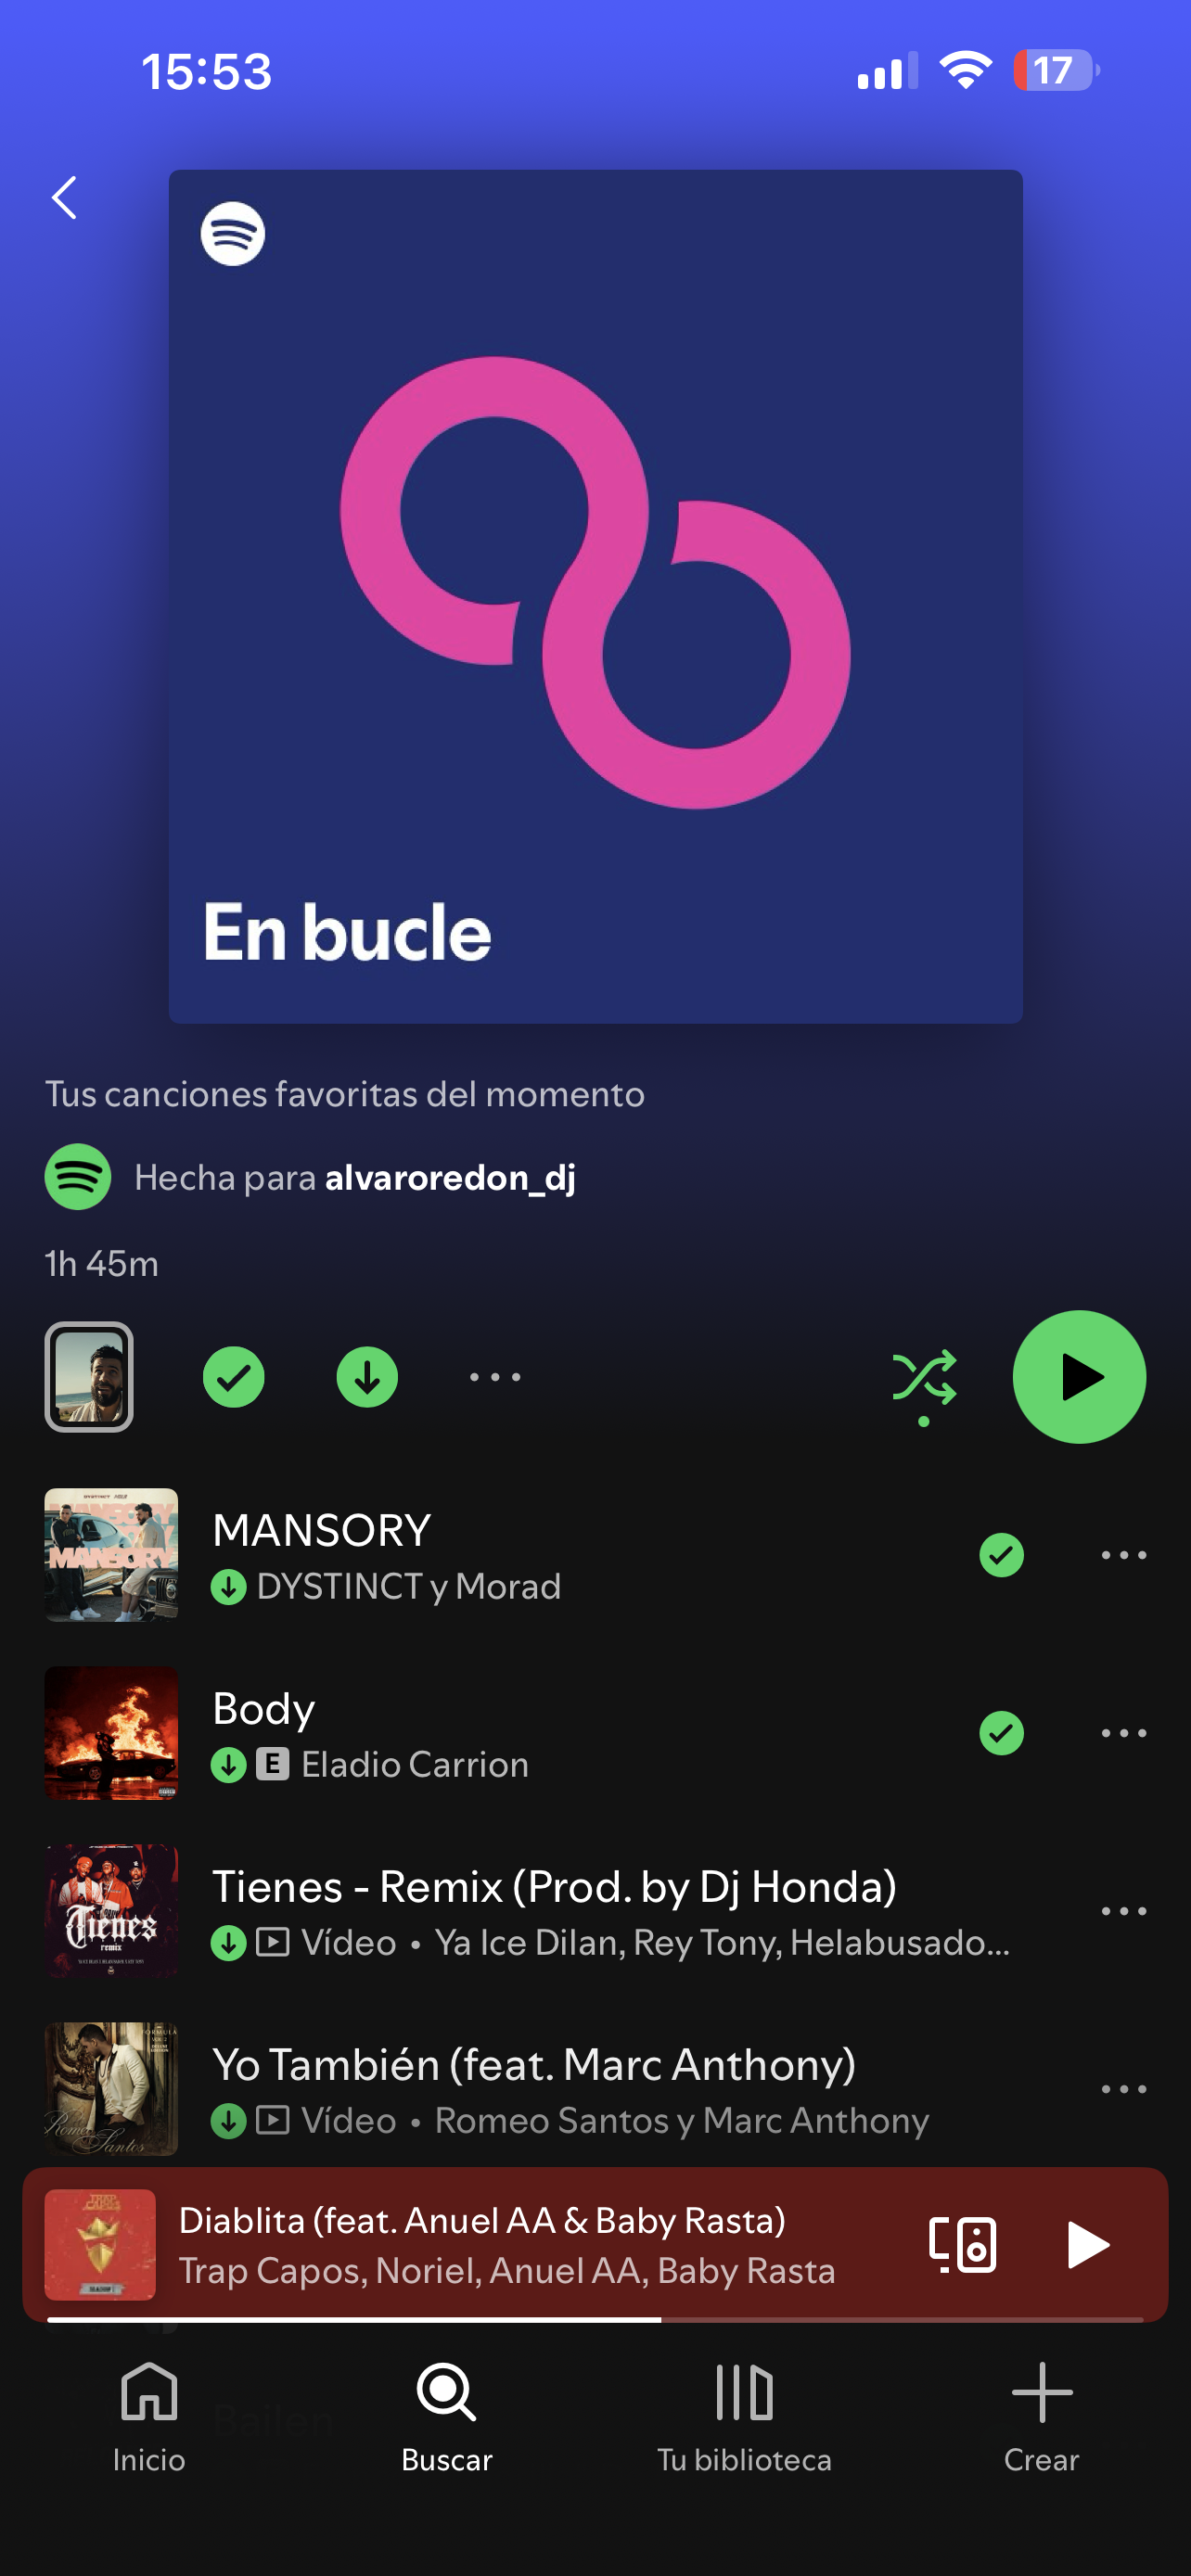
\includegraphics[width=\linewidth]{Imagenes/spotify.PNG}
    \caption{Spotify}
\end{subfigure}
\hfill
\begin{subfigure}[t]{0.24\textwidth}
    \centering
    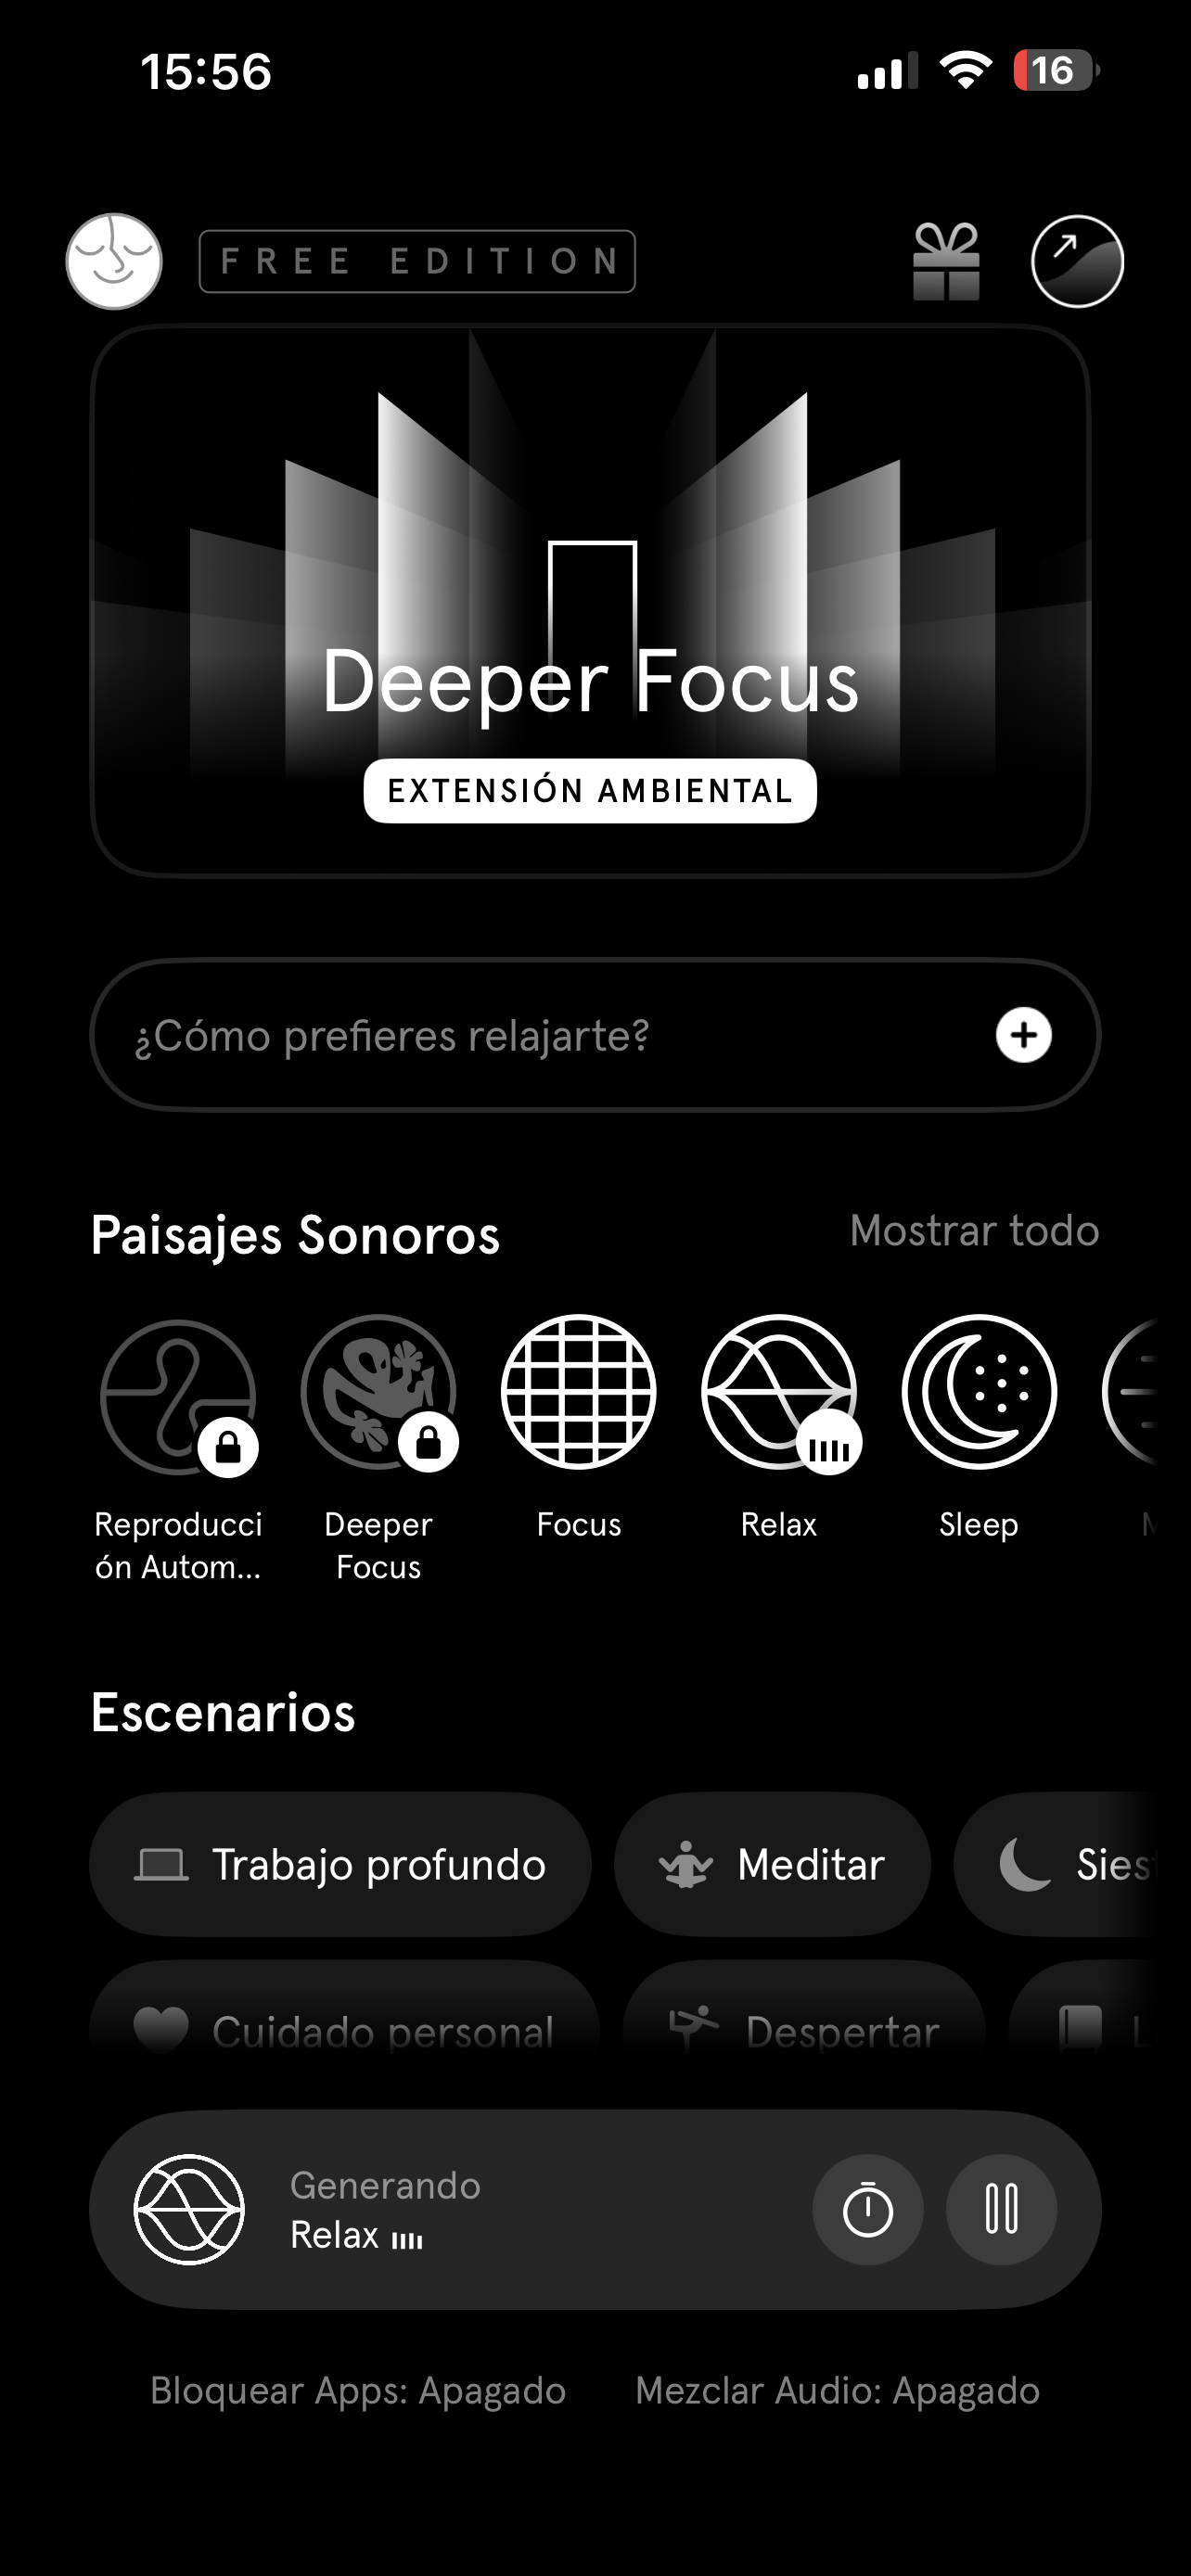
\includegraphics[width=\linewidth]{Imagenes/endel.PNG}
    \caption{Endel}
\end{subfigure}
\hfill
\begin{subfigure}[t]{0.24\textwidth}
    \centering
    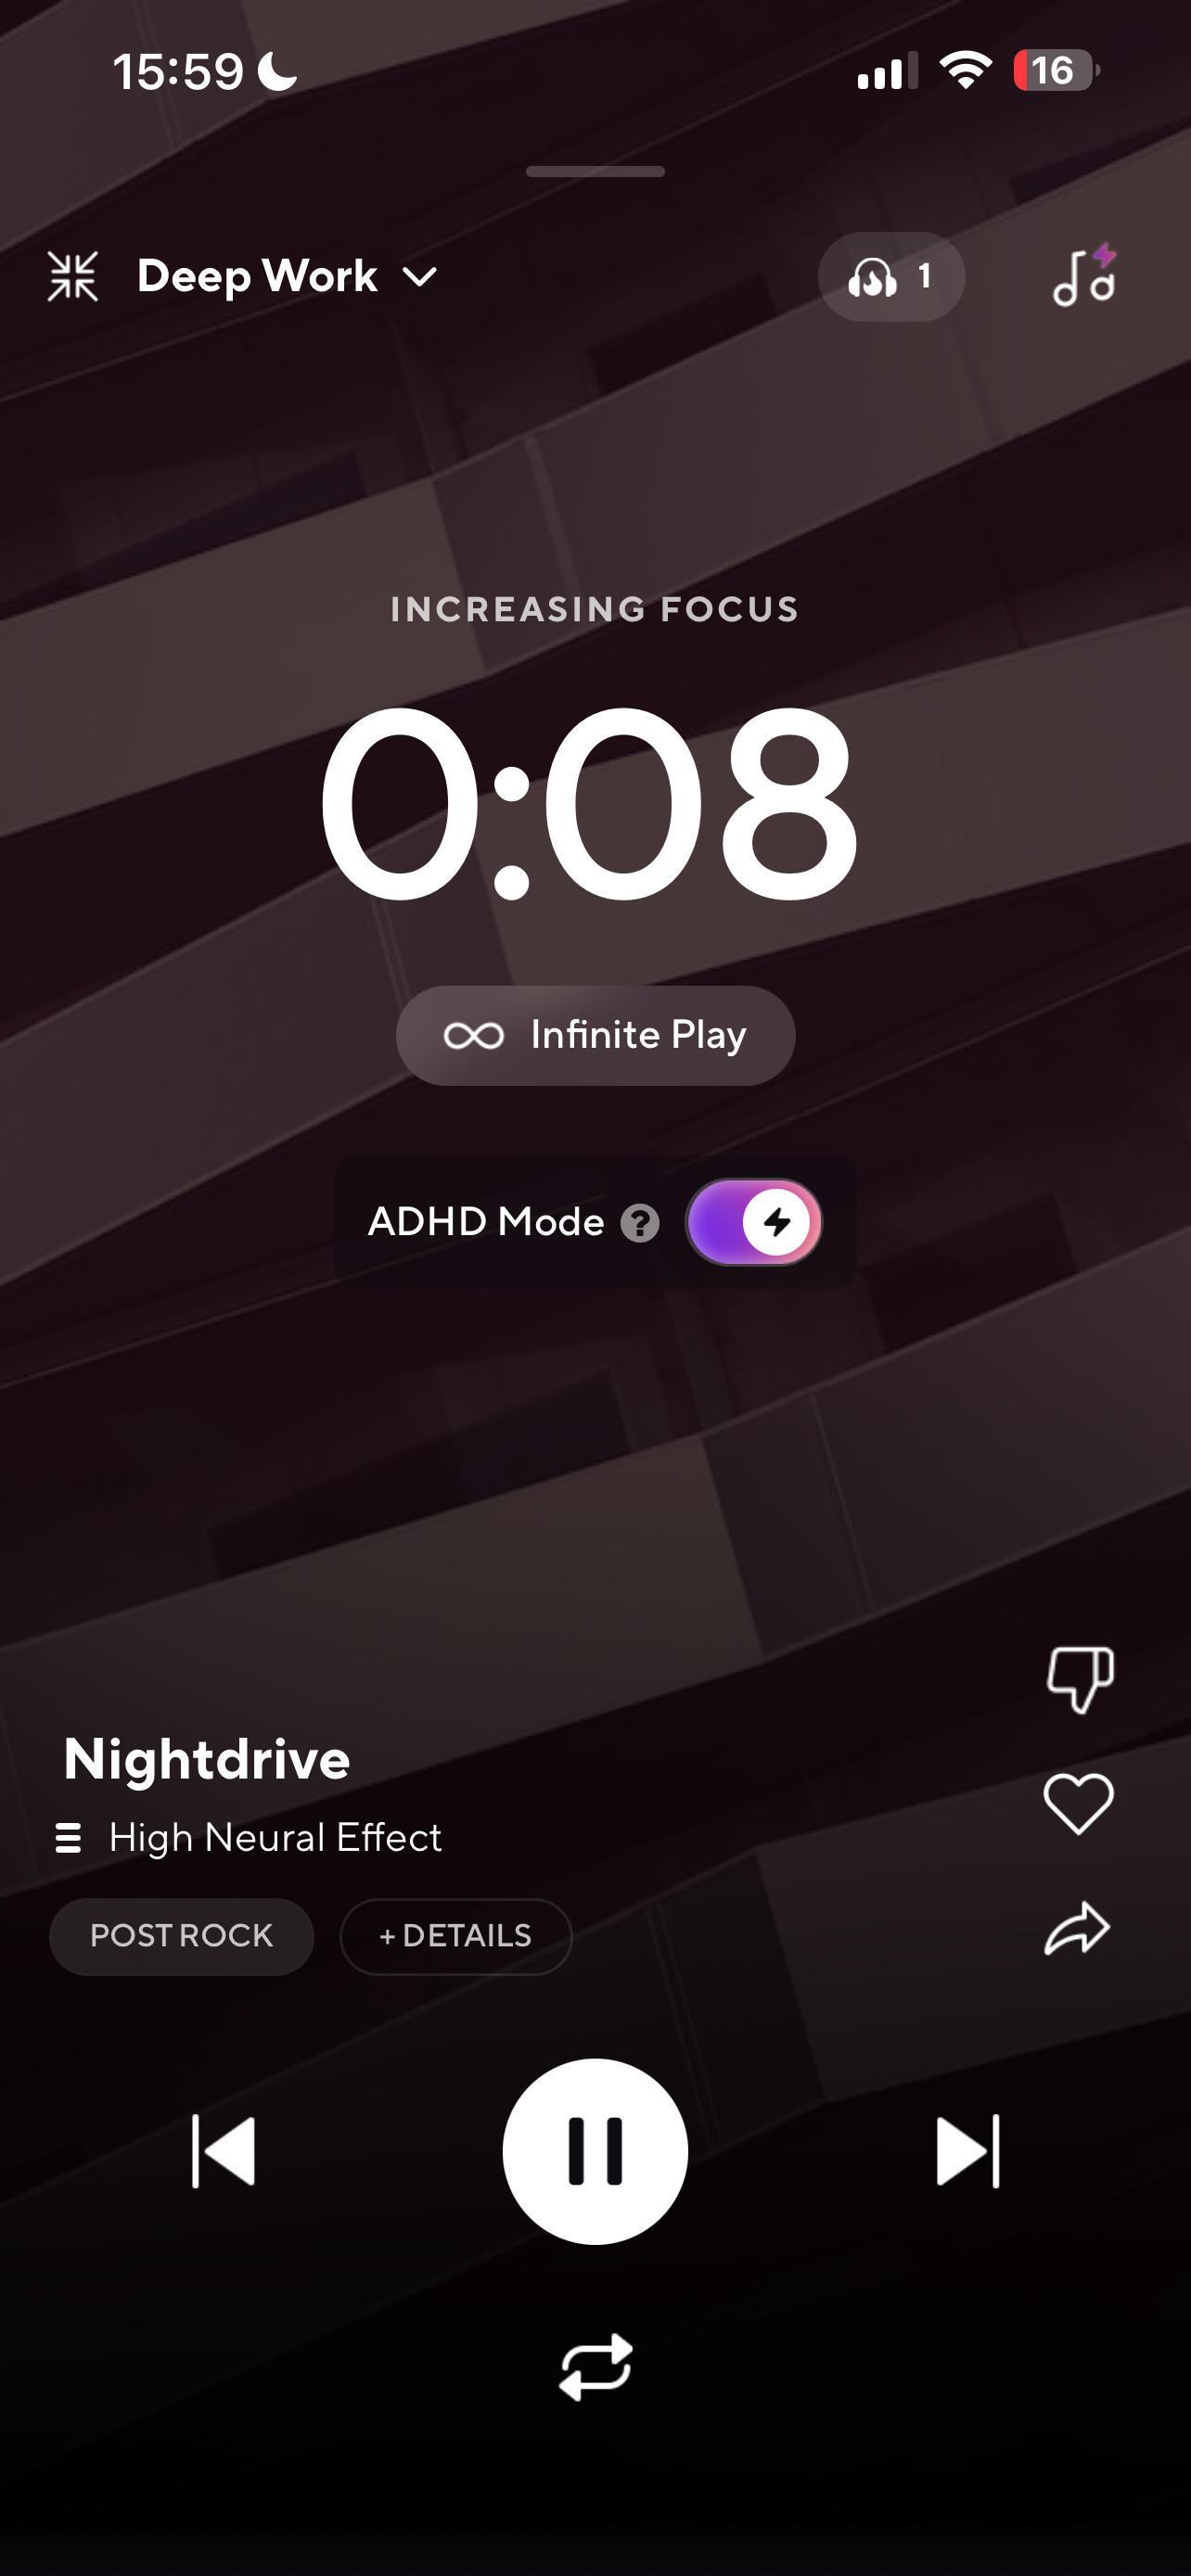
\includegraphics[width=\linewidth]{Imagenes/brainfm.PNG}
    \caption{Brain.fm}
\end{subfigure}
\hfill
\begin{subfigure}[t]{0.24\textwidth}
    \centering
    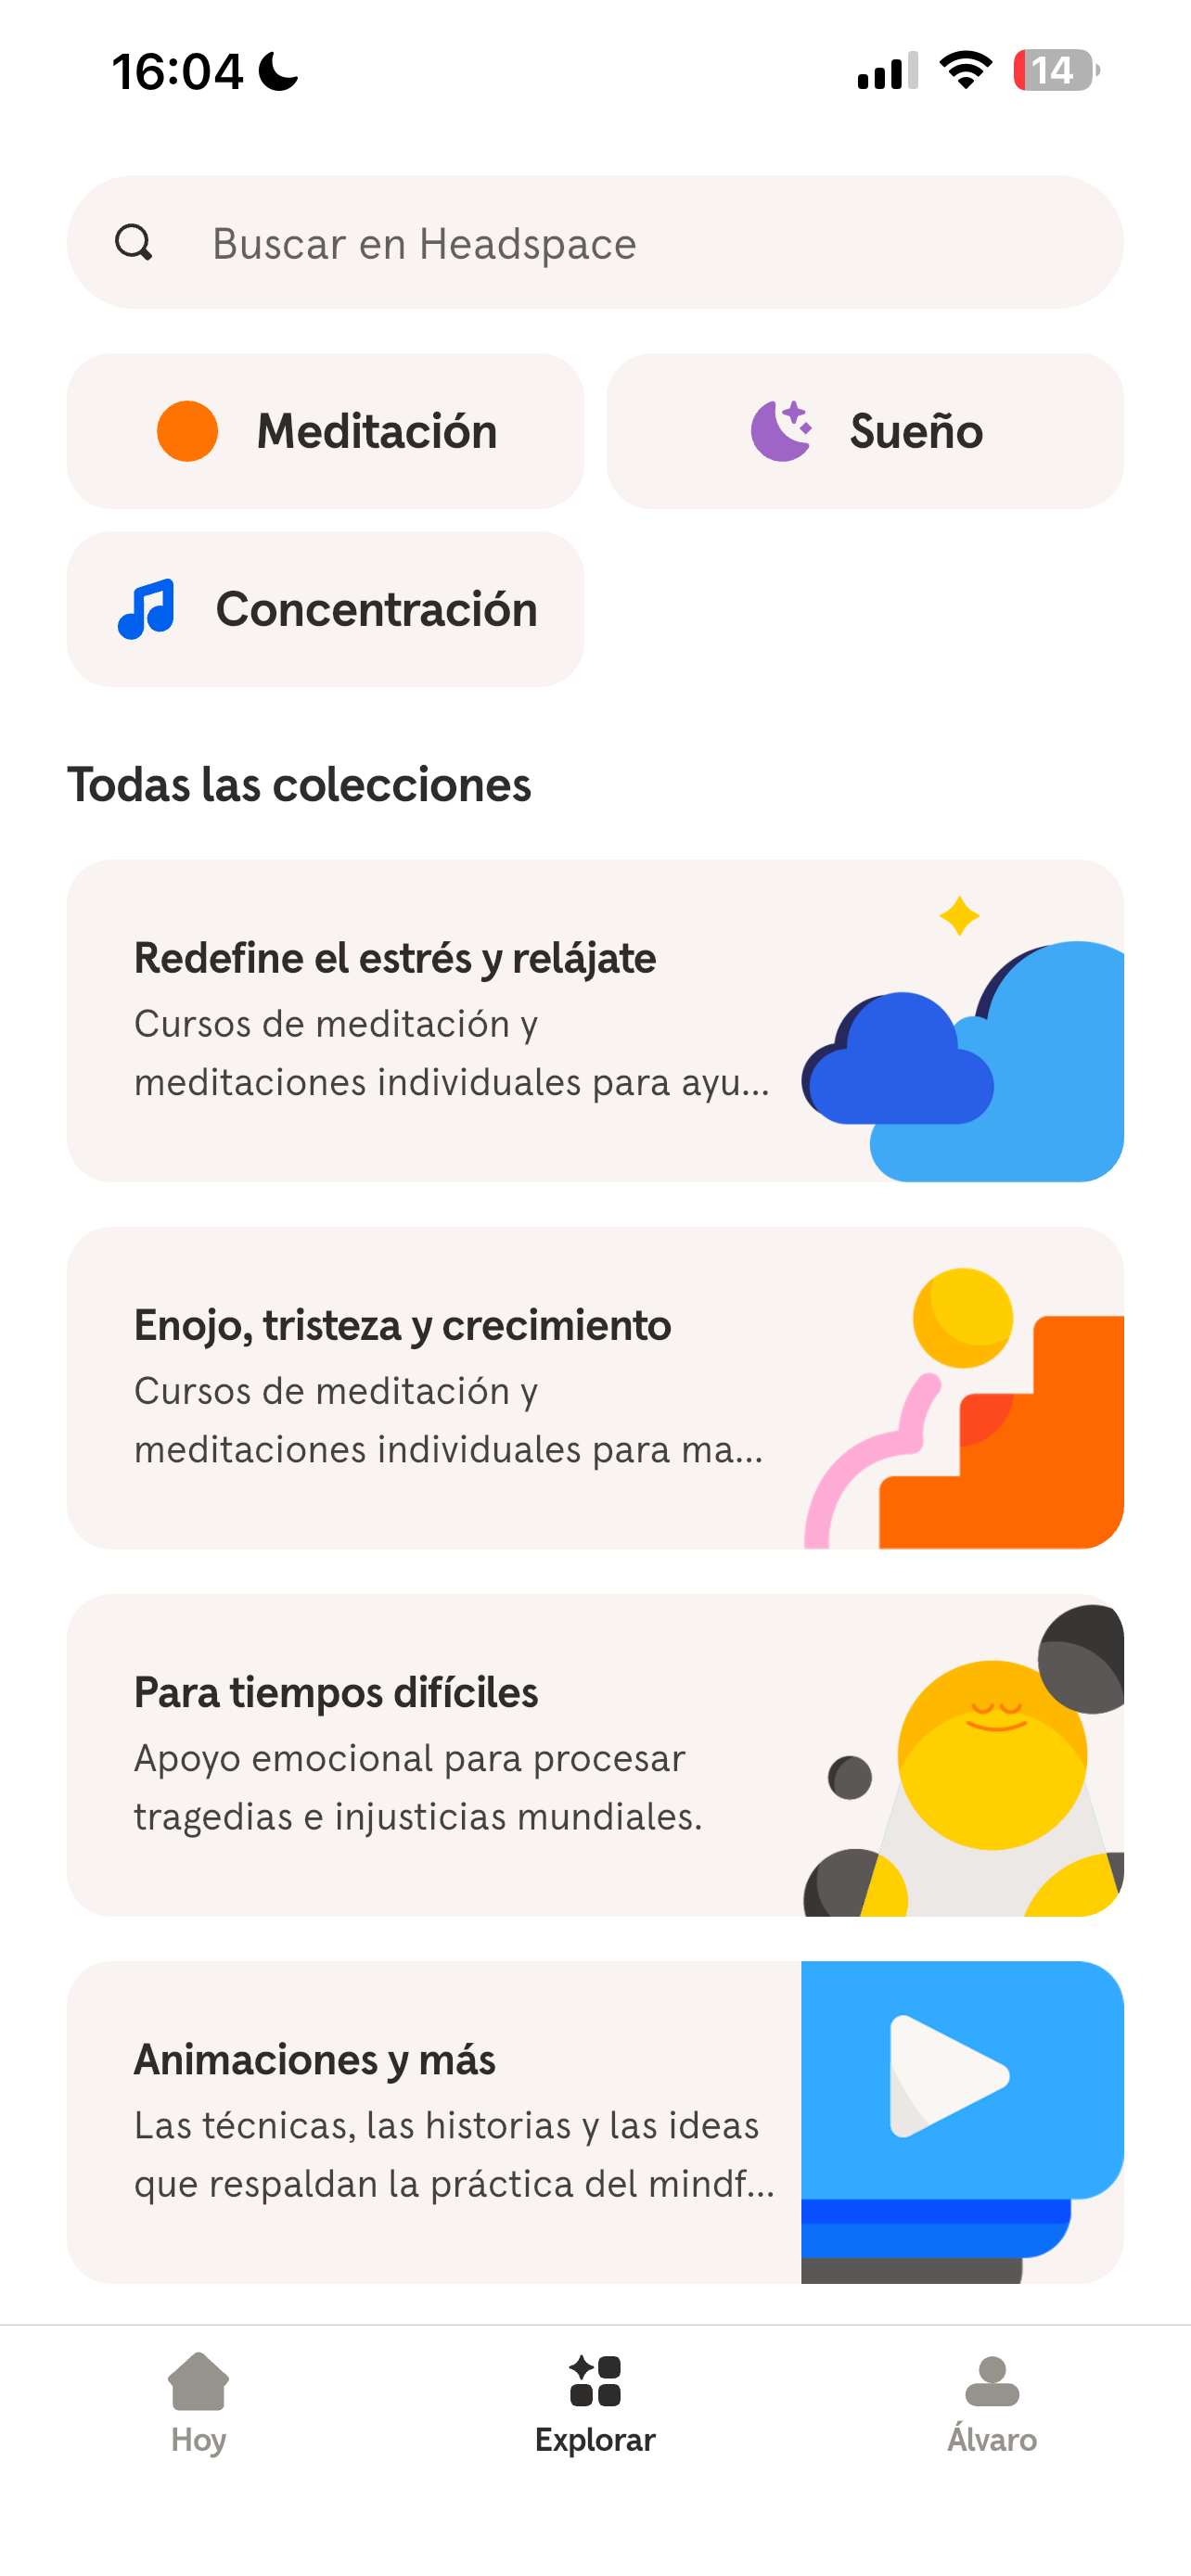
\includegraphics[width=\linewidth]{Imagenes/headspace.PNG}
    \caption{Headspace}
\end{subfigure}
\caption{Capturas representativas de soluciones relacionadas analizadas. Spotify destaca por la playlist personalizada; Endel por el paisaje sonoro adaptativo; Brain.fm por la sesión funcional orientada a foco; y Headspace por el ecosistema de bienestar con secciones de meditación, sueño y concentración.}
\label{fig:apps_relacionadas}
\end{figure}

La figura \ref{fig:apps_relacionadas} ayuda a aterrizar visualmente la comparación anterior. Spotify presenta una interfaz centrada en listas personalizadas y consumo musical habitual; Endel y Brain.fm muestran propuestas donde el audio se articula como sesión funcional o paisaje sonoro; y Headspace organiza la experiencia alrededor de categorías de bienestar como meditación, sueño o concentración. Esta lectura visual refuerza la idea de que Harmony Hub no replica ninguna de estas soluciones de forma directa, sino que toma elementos de varias de ellas para combinarlos en un flujo único con check-in, recomendación contextual, playlist real y feedback.

Vistas en conjunto, estas soluciones muestran que el problema que plantea Harmony Hub no parte de cero. Al contrario: se sitúa en un territorio donde ya existen muy buenas respuestas parciales. Spotify sobresale en personalización musical, Endel en adaptación contextual sonora, Brain.fm en audio funcional orientado a estados concretos y Headspace en experiencia de bienestar guiada. Precisamente por eso, la aportación del proyecto no consiste en negar esas referencias, sino en dialogar con ellas y proponer una combinación diferente favoreciendo al usuario en su bienestar personal.

\section{Evidencia sobre música y bienestar psicológico}
\label{sec:evidencia_musica_bienestar}

Además de las soluciones comerciales analizadas, existe una base académica que
justifica la relación entre música, bienestar y regulación psicológica. La
revisión de alcance de la OMS sobre artes y salud concluye que las actividades
artísticas, incluidas distintas formas de participación musical, pueden
contribuir a reducir malestar psicológico, depresión y ansiedad en diversos
grupos poblacionales \cite{who_arts_2019}. Esta evidencia no legitima por sí
sola cualquier sistema musical automatizado, pero sí apoya la idea de que la
música puede utilizarse como mediador relevante dentro de intervenciones de
bienestar cotidiano.

Un caso especialmente próximo al propósito de Harmony Hub es el ensayo
aleatorizado de Coulton et al. sobre canto comunitario en personas mayores. En
ese estudio, la participación en grupos de canto mostró mejoras en calidad de
vida relacionada con la salud mental y reducciones en ansiedad y depresión
frente a actividades habituales \cite{coulton_2015}. El interés de este
antecedente no reside en que Harmony Hub replique una intervención terapéutica
grupal, sino en que demuestra que una experiencia musical intencional, social y
estructurada puede producir beneficios psicológicos medibles cuando se diseña
alrededor de una necesidad humana concreta.

La conexión con este proyecto resulta directa. Harmony Hub no se plantea como
musicoterapia clínica ni como sustituto de acompañamiento profesional, pero sí
como una capa tecnológica capaz de acercar esa lógica de intencionalidad al uso
cotidiano de la música. En lugar de proponer escucha indiscriminada, el sistema
parte de un check-in explícito, modela el contexto inmediato y transforma esa
lectura en una sesión musical funcional orientada a foco, relajación,
acompañamiento o activación. Por ello, estos antecedentes refuerzan la
pertinencia del proyecto: sitúan la música no solo como entretenimiento, sino
como herramienta potencial de apoyo psicológico ligero y contextual.

\section{Comparativa}
\label{sec:comparativa}

\begin{table}[H]
\centering
\scriptsize
\renewcommand{\arraystretch}{1.1}
\setlength{\tabcolsep}{3pt}
\begin{tabularx}{\textwidth}{|P{1.85cm}|P{1.45cm}|P{1.65cm}|P{1.35cm}|P{1.65cm}|P{1.35cm}|Y|}
\hline
\textbf{Solución} & \textbf{Check-in contextual} & \textbf{Genera playlist real} & \textbf{Usa feedback} & \textbf{Aprende del historial} & \textbf{Usa entorno} & \textbf{Observación principal} \\
\hline
\textbf{Spotify} & No & Sí & Parcial & Sí & No & Personaliza muy bien la escucha, pero no parte de un estado emocional declarado ni cierra la sesión con una valoración explícita \cite{spotify_playlists,spotify_responsible_recs}. \\
\hline
\textbf{Endel} & Parcial & No & No & Parcial & Sí & Integra contexto y adaptación sonora, pero la salida son soundscapes propios, no playlists reproducibles en una cuenta de streaming \cite{endel_technology}. \\
\hline
\textbf{Brain.fm} & Parcial & No & No & Parcial & No & Está muy orientada a foco o relajación, pero opera sobre un catálogo funcional propio y no sobre la música cotidiana del usuario \cite{brainfm_official}. \\
\hline
\textbf{Headspace} & Parcial & No & Parcial & Parcial & No & Ofrece una experiencia de bienestar muy cuidada, pero no articula un flujo de recomendación musical contextualizada con playlists reales en Spotify \cite{headspace_focus}. \\
\hline
\textbf{Harmony Hub} & Sí & Sí & Sí & Sí & Sí & Integra check-in, recomendación de sesión, playlist real, historial y aprendizaje progresivo dentro de un mismo flujo de uso, con abstención controlada del componente aprendido cuando no hay evidencia suficiente. \\
\hline
\end{tabularx}
\caption{Comparativa funcional entre soluciones relacionadas y Harmony Hub.}
\label{tab:comparativa_soluciones}
\end{table}

La tabla anterior permite observar mejor el hueco que intenta cubrir Harmony
Hub. No se trata de que las demás soluciones sean incompletas en sentido
absoluto, sino de que cada una resuelve muy bien una parte distinta del
problema. La aportación del proyecto aparece precisamente al combinar en un
mismo flujo un check-in explícito, una recomendación contextual, la
materialización en Spotify y un cierre mediante feedback reutilizable.

\section{Justificación de la solución propuesta}
\label{sec:justificacion_solucion}

La comparación anterior permite justificar la pertinencia de Harmony Hub. El proyecto no pretende sustituir a Spotify como plataforma de consumo musical ni competir con Endel, Brain.fm o Headspace en sus respectivos nichos. Su aportación consiste en construir una capa intermedia entre la situación del usuario y la reproducción musical efectiva.

Esa capa intermedia se apoya en varios elementos que, combinados, diferencian la propuesta. En primer lugar, introduce un \textbf{check-in breve y contextual} que obliga al sistema a mirar el momento presente, y no solo el historial acumulado. En segundo lugar, convierte esa lectura en una \textbf{recomendación de sesión} que luego puede materializarse en una \textbf{playlist real dentro de Spotify}, algo importante porque evita que la experiencia se quede en una simulación o en un entorno sonoro aislado. En tercer lugar, sostiene la recomendación musical sobre un \textbf{catálogo estructurado propio}, lo que mejora trazabilidad y estabilidad frente a depender por completo de búsquedas abiertas en una API externa. En cuarto lugar, incorpora \textbf{historial y feedback} para cerrar el ciclo de uso y permitir un aprendizaje progresivo del sistema. Y, además, ese aprendizaje no se aplica de forma ciega: queda condicionado por evidencia suficiente y por puertas de calidad que reducen el riesgo de sobreinterpretar señales débiles o demasiado escasas.

La solución resulta especialmente adecuada como Trabajo Fin de Grado porque integra varias dimensiones de la ingeniería de software en un problema real: diseño de interacción, arquitectura cliente-servidor, persistencia, integración con APIs externas, trazabilidad de sesiones y un componente de aprendizaje supervisado evaluable con métricas objetivas cuando el volumen de datos lo permite.

En definitiva, Harmony Hub se justifica no porque el mercado carezca de herramientas musicales o de bienestar, sino porque todavía hay margen para propuestas que unan mejor ambos mundos. Y esa unión, en este caso, se articula alrededor de una idea sencilla pero con bastante potencial: usar la música no solo como contenido que acompaña, sino como respuesta intencional a un momento concreto de la vida cotidiana.
